\documentclass[12pt,a4paper]{article}
\usepackage[utf8]{inputenc}
\usepackage[russian]{babel}
\usepackage[OT1]{fontenc}
\usepackage{amsmath}
\usepackage{amsfonts}
\usepackage{amssymb}
\usepackage{graphicx}
\usepackage{array}
\usepackage{cancel}
\usepackage{caption}
\usepackage{wrapfig}
\usepackage{secdot}
\usepackage{indentfirst}
\usepackage[left=1.5cm,right=1.5cm,top=0.3cm,bottom=1.5cm,includefoot,footskip=1.5cm]{geometry}
\begin{document}
\textbf{
\begin{flushright}
Илья Кочергин, 626 группа
\end{flushright}}
\begin{flushleft}
\large\textbf{Работа 3.2.6}
\medskip

\Large\textbf{Исследование гальванометра}
\end{flushleft}

\noindent\textbf{Цель работы:} изучение работы высокочувствительного магнитозеркального гальванометра магнитоэлектрической системы в режимах измерения постоянного тока и электрического заряда.
\medskip

\noindent\textbf{Оборудование:} зеркальный гальванометр с осветителем и шкалой, источник постоянного напряжения, делитель напряжения, магазин сопротивлений, эталонный конденсатор, вольтметр, переключатель, ключ, линейка.

\section{Теоретическая справка}
\begin{wrapfigure}{r}{0.23\textwidth}
\centering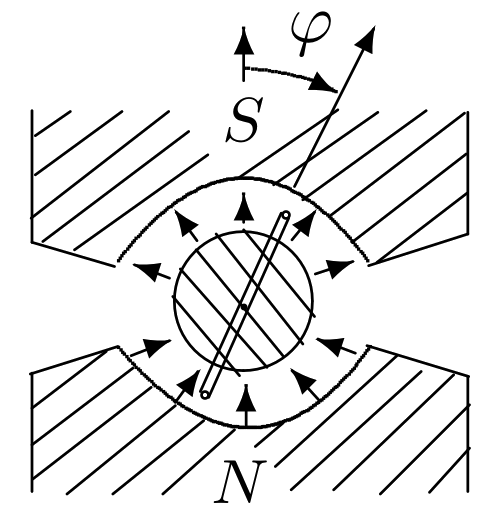
\includegraphics[width = 0.17\textwidth]{Pct1}
\captionsetup{justification = centering}
\caption{Рамка с током в магнитном поле \label{Fig1}}
\end{wrapfigure}
\textbf{Устройство.} Баллистический гальванометр - электроизмерительный прибор магнитоэлектрической системы, отличающийся высокой чувствительностью и сравнительно большим периодом колебаний подвижной части. Он представляет собой скрепленную с полым цилиндром проводящую рамку, подвешенную на нити в радиально направленном постоянном магнитном поле (см. рис. \ref{Fig1}). На рамке закреплено зеркало, служащее для измерения угла поворота.
\medskip

\textbf{Уравнение движения.} Введем следующие обозначения: $\varphi$ - угол поворота рамки, $D$ - модуль кручения, $S$ - площадь рамки, $N$ - число витков, $I$ - сила тока в рамке при отсутствии ЭДС индукции, $B$ - индукция магнитного поля, $R_{\Sigma}$ - общее сопротивление цепи, $J$ - момент инерции подвижной системы. Если пренебречь сопротивлением воздуха, то уравнение движения записывается в виде
\begin{equation}
J\ddot\varphi + \frac{(BSN)^2}{R_{\Sigma}}\dot\varphi + D\varphi = BSNI\label{em}.
\end{equation}
Введем обозначения
\begin{equation}
\begin{cases}
2\gamma = \frac{(BSN)^2}{JR_{\Sigma}},\\
\omega_0^2 = \frac{D}{J},\\
K = \frac{BSN}{J}.\\ 
\end{cases}\label{redef}
\end{equation}
Таким образом, уравнение (\ref{em}) примет вид
\begin{equation}
\ddot\varphi + 2\gamma\dot\varphi + \omega_0^2\varphi = KI\label{emm}.
\end{equation}
Заметим, что данное уравнения является уравнением затухающих колебаний с коэффициентом затухания $\gamma$ и собственной частотой $\omega_0$.
\medskip

\textbf{Режим измерения постоянного тока.} Если $I = const$, то по прошествии некоторого времени колебания затухнут, и можно принять $\varphi = const$. Тогда из уравнения (\ref{emm}) легко получить
\begin{equation}
\varphi = \frac{K}{\omega_0^2}I = \frac{BSN}{D}I = \frac{I}{C_I}.
\end{equation}
$C_I$ называется \textit{динамической постоянной} гальванометра и определяется выражением
\begin{equation}
C_I = \frac{I}{\varphi} = \frac{D}{BSN}.\label{dyn}
\end{equation}
\medskip

\textbf{Свободные колебания рамки.} Пусть $I = 0$ и выполнены следующие начальные условия:
\begin{equation}
\begin{cases}
\varphi(t = 0) = 0,\\
\dot\varphi(t = 0) = \dot\varphi_0.\\
\end{cases}
\end{equation}
Тогда в зависимости от $\gamma$ и $\omega_0$ решение уравнения (\ref{emm}) имеет вид
\begin{equation}
\begin{cases}
\varphi = \frac{\dot\varphi_0}{\omega}e^{-\gamma t}\sin\omega t,&\gamma < \omega_0~\text{(колебательный режим)};\\
\varphi = \dot\varphi_0te^{-\gamma t},&\gamma = \omega_0~\text{(критический режим)};\\
\varphi = \frac{\dot\varphi_0}{\varkappa}e^{-\gamma t}\sh\varkappa t,&\gamma > \omega_0~\text{(апериодический режим)}.\\
\end{cases}\label{sol}
\end{equation}
Здесь $\varkappa$ и $\omega$ определяются соотношениями
\begin{equation}
\begin{cases}
\omega^2 = \omega_0^2 - \gamma^2,\\
\varkappa^2 = \gamma^2 - \omega_0^2.\\
\end{cases}\label{omega}
\end{equation}

В случае колебательного режима можно ввести логарифмический декремент затухания $\Theta$:
\begin{equation}
\Theta = \ln\frac{\varphi_n}{\varphi_{n+1}},
\end{equation}
где $\varphi_n$ и $\varphi_{n+1}$ - углы последовательных отклонений в одну сторону с номерами $n$ и $n+1$. Из (\ref{sol}) в случае малого затухания ($\gamma \ll \omega$) легко получить выражение для $\Theta$:
\begin{equation}
\Theta = \gamma T\label{decr},
\end{equation}
где $T$ - период колебаний:
\begin{equation}
T = \frac{2\pi}{\omega}\label{per}.
\end{equation}
Заметим, что при приближении к критическому режиму $\Theta \to \infty$.
\medskip

\textbf{Режим измерения заряда.} Теперь рассмотрим ситуацию, когда через гальванометр проходит короткий импульс тока. Будем считать, что продолжительность импульса $\tau$ достаточно мала ($\tau \ll T$), и отклонением рамки можно пренебречь. Пусть через рамку протекал ток с момента времени $t = 0$ до момента времени $t = \tau$. Проинтегрировав уравнение (\ref{emm}) с учетом приближения $\varphi \approx 0$, получим
\begin{equation}
\dot\varphi(\tau) = K\int\limits_0^\tau Idt\label{dotphi1}.
\end{equation}
Заряд, прошедший через гальванометр выражается формулой
\begin{equation}
q = \int\limits_0^\tau Idt + \int\limits_0^\tau I_{\text{инд}}dt\label{ch},
\end{equation}
где $I_{\text{инд}}$ - индукционный ток. Заметим, что $I_{\text{инд}} \sim \dot\varphi$, а значит
\begin{equation}
\int\limits_0^\tau I_{\text{инд}}dt \sim \int\limits_0^\tau \dot\varphi dt = \varphi(\tau) \approx 0.
\end{equation}
Поэтому зарядом, протекшим в результате индукционного тока, можно пренебречь, и выражение (\ref{ch}) примет вид
\begin{equation}
q = \int\limits_0^\tau Idt.
\end{equation}
Отсюда и из выражения (\ref{dotphi1}) получим
\begin{equation}
\dot\varphi(\tau) = Kq\label{dotphi2}.
\end{equation}
Из выражения (\ref{sol}) легко видеть, что при любом режиме максимальное отклонение от положения равновесия $\varphi_\text{max} \sim \dot\varphi_0 \stackrel{(\ref{dotphi2})}{\sim} q$. Таким образом, величина
\begin{equation}
C_q = \frac{q}{\varphi_\text{max}}\label{bal},
\end{equation}
называемая \textit{баллистической постоянной}, зависит только от параметров цепи.

Можно показать, что при неизменном $q$ максимальное отклонение достигается при отсутствии затухания и определяется выражением
\begin{equation}
\varphi_{\text{max св}} = \frac{\dot\varphi(\tau)}{\omega_0} = \frac{Kq}{\omega_0}\label{fr}.
\end{equation}
В критическом режиме, когда система быстрее всего приходит в равновесие, максимальное отклонение в $e$ раз меньше:
\begin{equation}
\varphi_{\text{max кр}} = \frac{Kq}{\omega_0e}\label{cr}.
\end{equation}
Отсюда следует выражение для баллистических констант:
\begin{equation}
\frac{C_{Q\text{ кр}}}{C_{Q\text{ св}}} = e\label{rat}.
\end{equation}

\section{Определение динамической постоянной}
\begin{wrapfigure}{r}{0.5\textwidth}
\centering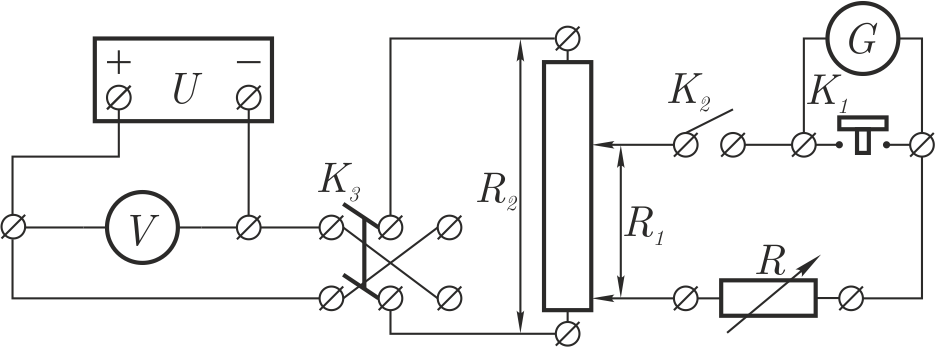
\includegraphics[width = 0.47\textwidth]{Sch1}
\captionsetup{justification = centering}
\caption{Схема установки для работы в стационарном режиме \label{Fig2}}
\end{wrapfigure}
\textbf{Экспериментальная установка.} Схема для измерений в стационарном режиме приведена на рис. \ref{Fig2}. Значение входного напряжения $U = 1,32 \pm 0,02~\text{В}$, сопротивления гальванометра $R_0 = 475 \pm 1~\text{Ом}$. Сопротивление $R$ можно изменять.

Угол отклонения рамки от положения равновесия измеряется с помощью осветителя, зеркала, закрепленного на рамке, и шкалы, на которую отражается свет. Если обозначить координату светового пятна за $x$ и считать $x \ll a$, то выражение для угла отклонения примет вид
\begin{equation}
\varphi = \frac{x}{2a},
\end{equation}
где $a = 128 \pm 1~\text{см}$ - расстояние от шкалы до зеркала. Таким образом, из выражения (\ref{dyn}) легко получить формулу для динамической постоянной:
\begin{equation}
C_I = \frac{2aI}{x} 
\end{equation}
Отсюда следует выражение для зависимости $I(x)$:
\begin{equation}
I = x\frac{C_I}{2a}\label{dyn_rel}.
\end{equation}

При $R_1 \ll R + R_0$ сила тока, протекающего через гальванометр, выражается формулой
\begin{equation}
I = U\frac{R_1}{R_2}\frac{1}{R + R_0}.
\end{equation}
По этой формуле мы можем рассчитать токи по значениям сопротивления $R$, и, таким образом, получить экспериментальную зависимость $I(x)$. Согласно (\ref{dyn_rel}), она должна быть линейной, и по ее коэффициенту наклона $k$ мы сможем вычислить $C_I$:
\begin{equation}
C_I = 2ka.\label{dyn_exp}
\end{equation}
\medskip

\textbf{Обработка результатов.} Экспериментальные данные вместе с пересчитанными значениями занесены в таблицу \ref{tab1}.
\begin{table}[h!]\centering
\begin{tabular}{|*{10}{c|}}
\hline
$R,~\text{кОм}$&90&80&70&60&50&40&30&25&23\\
\hline
$x,~\text{см}$&5,6&6,3&7,2&8,3&10&12,6&16,9&20,3&22,2\\
\hline
$I, \text{нА}$&7,3&8,2&9,4&10,9&13,1&16,3&21,7&25,9&28,1\\
\hline
$\Delta I, \text{нА}$&0,1&0,1&0,1&0,2&0,2&0,2&0,3&0,4&0,4\\
\hline
\end{tabular}
\caption{Данные для измерения $C_I$ \label{tab1}}
\end{table}

\noindent Здесь $\Delta I$ - погрешность силы тока, вычисляемая по формуле
\begin{equation}
\Delta I = \frac{\Delta U}{U},
\end{equation}
т,к, сопротивление $R_0$ мало по сравнению с $R$, и мы считаем, что сопротивление магазина измеряется точно. За погрешность измерения $x$ принимается $\Delta x = 0,05~\text{см}$.

\begin{figure}[h!]\centering
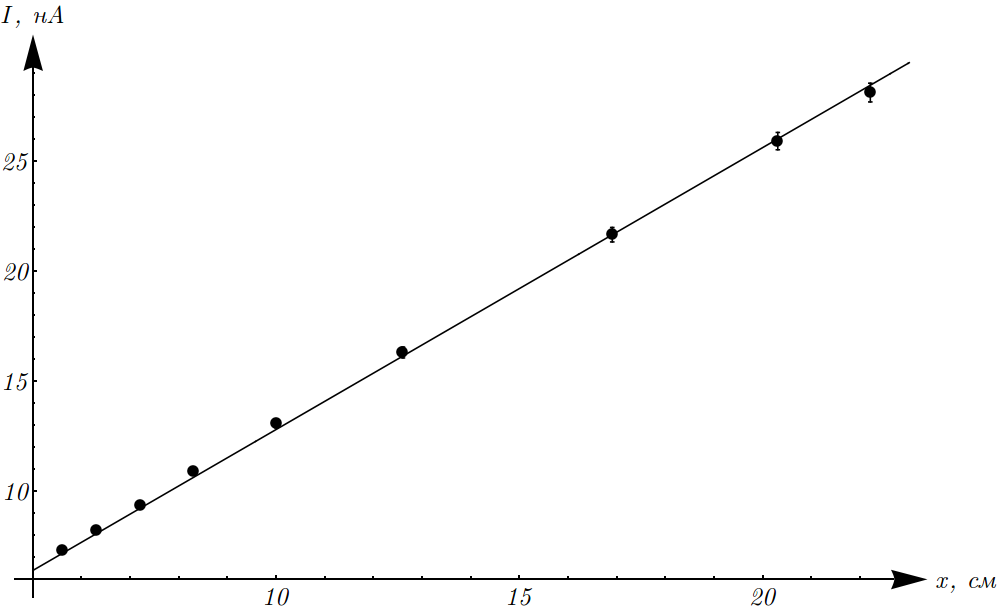
\includegraphics[width = 0.9\textwidth]{Plot1}
\captionsetup{justification = centering}
\caption{График зависимости $I(x)$ \label{Fig3}}
\end{figure}

По этим данным построим график зависимости $I(x)$, он изображен на рис. \ref{Fig3}. Из графика находим значение коэффициента наклона:
\begin{equation}
k = (1,28 \pm 0,01)\cdot10^{-7}~\text{А/м}.
\end{equation}
Отсюда по формуле (\ref{dyn_exp}) находим значение $C_I$:
\begin{equation}
C_I = (3,28 \pm 0,04)\cdot10^{-7}~\text{А},
\end{equation}
погрешность $C_I$ была вычислена по формуле
\begin{equation}
\Delta C_I = C_I\sqrt{\left(\frac{\Delta a}{a}\right)^2 + \left(\frac{\Delta k}{k}\right)^2}.
\end{equation}
\section{Определение~критического~сопротивления~гальванометра} 
\textbf{Экспериментальная установка.} В этой части измерения проводятся на той же схеме,~что и~в~предыдущей, но при свободных колебаниях рамки.

При достаточно больших $R$ из (\ref{redef}) следует, что $\gamma < \omega_0$ и, согласно (\ref{sol}), наблюдается колебательный режим. С уменьшением $R$ затухание увеличивается, и при $R = R_{\text{кр}}$ движение рамки переходит в критический режим. При $R > R_{\text{кр}}$ движение апериодическое.

Выразим логарифмический декремент затухания через параметры цепи. Подставляя в (\ref{decr}) выражения для периода из (\ref{per}), $\omega$ из (\ref{omega}),  $\gamma$ и $\omega_0$ из (\ref{redef}), находим:
\begin{equation}
\Theta = \frac{2\pi R_3}{\sqrt{{(R+R_0)}^2-R_3^2}},\label{decr_exp1}
\end{equation}
где $R_3$ определяется выражением
\begin{equation}
R_3 = \frac{\left(BSN\right)^2}{2\sqrt{JD}}.\label{r3}
\end{equation}
Для измерения $\Theta$ мы будем измерять начальное отклонение луча $x_0$ и отклонение после одного колебания $x_1$. Тогда логарифмический декремент затухания определяется выражением
\begin{equation}
\Theta = \ln\frac{x_0}{x_1}.\label{decr_exp_d}
\end{equation}

Теперь преобразуем равенство (\ref{decr_exp1}):
\begin{equation}
\frac{1}{\Theta^2}=\frac{\left(R_0+R\right)^2}{4\pi^2R_3^2} - \frac{1}{4\pi^2}.\label{decr_exp2}
\end{equation}
Отсюда график зависимости $\frac{1}{\Theta^2}\left(\left(R_0+R\right)^2\right)$ должен быть линеен, и его коэффициент наклона определяется выражением
\begin{equation}
k = \frac{1}{4\pi^2R_3^2}.\label{k_crit}
\end{equation}

Нам осталось выразить $R_3$ через известные параметры схемы и $R_\text{кр}$. Для этого вспомним, что при приближении к критическому режиму, то есть при $R\to R_\text{кр}$, $\Theta\to\infty$. Отсюда и из выражения (\ref{decr_exp1}) легко получить формулу для $R_3$:
\begin{equation}
R_3 = R_0 + R_\text{кр}.\label{r_3}
\end{equation}
Окочательно, подставив результат в (\ref{k_crit}), получим выражение для $R_\text{кр}:$
\begin{equation}
R_\text{кр} = \frac{1}{2\pi\sqrt{k}} - R_0.\label{r_crit}
\end{equation}

\textbf{Обработка результатов.} Сначала оценим $R_\text{кр}$. Для этого подберем наибольшее значение $R_\text{кр}$, при котором колебаний еще не наблюдается. Получим
\begin{equation}
R_\text{кр} \approx 9,1 \pm 0,2~\text{кОм}.
\end{equation}
Погрешность была оценена по минимальному изменению сопротивления, при котором заметно отличие в характере колебаний.

Теперь определим $R_\text{кр}$ из графика. Для того, чтобы можно было вычислять $\Theta$ с достаточной точностью, будем проводить измерения при $R \geq 3R_\text{кр}$. Экспериментальные данные вместе с пересчитанными значениями занесены в таблицу \ref{tab2}.
\begin{table}[ht]\centering
\begin{tabular}{|*{8}{c|}}
\hline
$R,~\text{кОм}$&30&33&36&39&42&45&48\\
\hline
$x_0,~\text{см}$&16,9&15,4&15,4&17,0&24,0&22,1&20,7\\
\hline
$x_1,~\text{см}$&2,1&2,5&3,2&3,9&5,7&6,2&6,3\\
\hline
$\frac{1}{\Theta^2}$&0,23&0,30&0,41&0,46&0,48&0,62&0,71\\
\hline
$\Delta\Theta^2$&0,02&0,02&0,03&0,02&0,02&0,02&0,02\\
\hline
$\left(R+R_0\right)^2,~\text{Ом}^2\cdot10^8$&9,29&11,21&13,30&15,58&18,04&20,68&23,50\\
\hline
$R,~\text{кОм}$&51&54&60&70&80&90&-\\
\hline
$x_0,~\text{см}$&20,5&18,3&16,5&23,2&20,3&18,0&-\\
\hline
$x_1,~\text{см}$&6,7&6,1&6,3&10,3&9,5&9,7&-\\
\hline
$\frac{1}{\Theta^2}$&0,80&0,83&1,08&1,52&1,73&2,62&-\\
\hline
$\Delta\Theta^2$&0,03&0,03&0,04&0,03&0,04&0,06&-\\
\hline
$\left(R+R_0\right)^2,~\text{Ом}^2\cdot10^8$&26,50&29,68&36,57&49,67&64,76&81,86&-\\
\hline
\end{tabular}
\caption{Данные для измерения $R_\text{кр}$ \label{tab2}}
\end{table}
По эти данным построим график требуемой зависимости (рис. \ref{Fig4})
\medskip

\begin{figure}[h]\centering
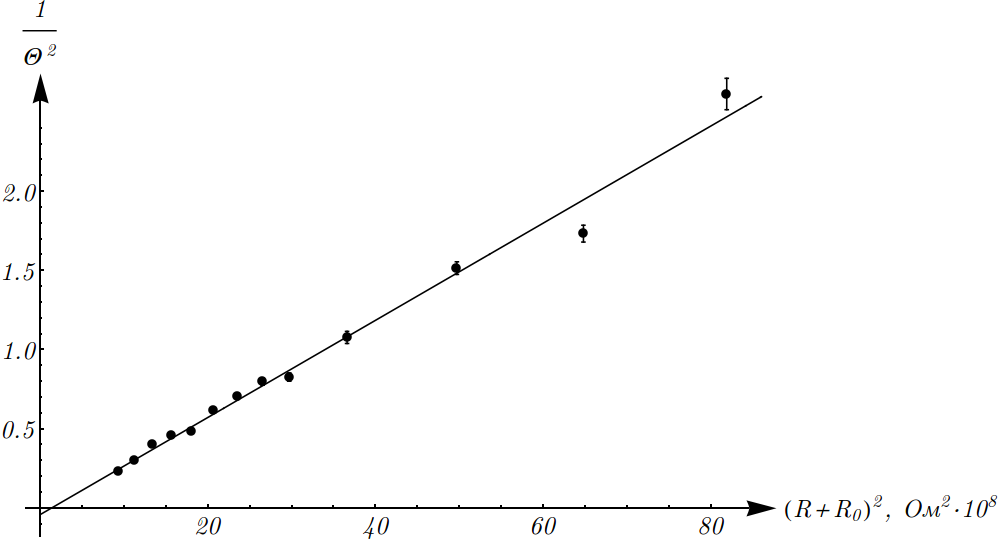
\includegraphics[width = 1\textwidth]{Plot2}
\captionsetup{justification = centering}
\caption{График зависимости $\frac{1}{\Theta^2}\left(\left(R_0+R\right)^2\right)$ \label{Fig4}}
\end{figure}

Из графика по МНК определим коэффициент наклона:
\begin{equation}
k \approx (0,31\pm0,01)\cdot 10^{-9}~\text{Ом}^{-2}.\label{k_val}
\end{equation}
Таким образом, по формуле (\ref{r_crit}) получаем искомое значение:
\begin{equation}
R_\text{кр} \approx (8,6 \pm 0,3)\text{кОм}.
\end{equation}

Здесь в таблице \ref{tab2} погрешности $x_0$ и $x_1$ принимались
\begin{equation}
\Delta x_0 = \Delta x_1 = \Delta x = 0,2~\text{см},
\end{equation}
погрешность $\frac{1}{\Theta^2}$ вычислялась по формуле
\begin{equation}
\Delta \frac{1}{\Theta^2} = \frac{\Delta x\sqrt{\frac{1}{x_0^2} + \frac{1}{x_1^2}}}{\Theta}\frac{1}{\Theta^2},
\end{equation}
погрешность измерения сопротивления считалась малой, а погрешность $R_\text{кр}$ вычислялась по формуле
\begin{equation}
\Delta R_\text{кр} = \frac{\Delta k}{k}R_\text{кр}.
\end{equation}
\section{Определение баллистической постоянной и критического сопротивления гальванометра.}
\begin{wrapfigure}{r}{0.49\textwidth}
\centering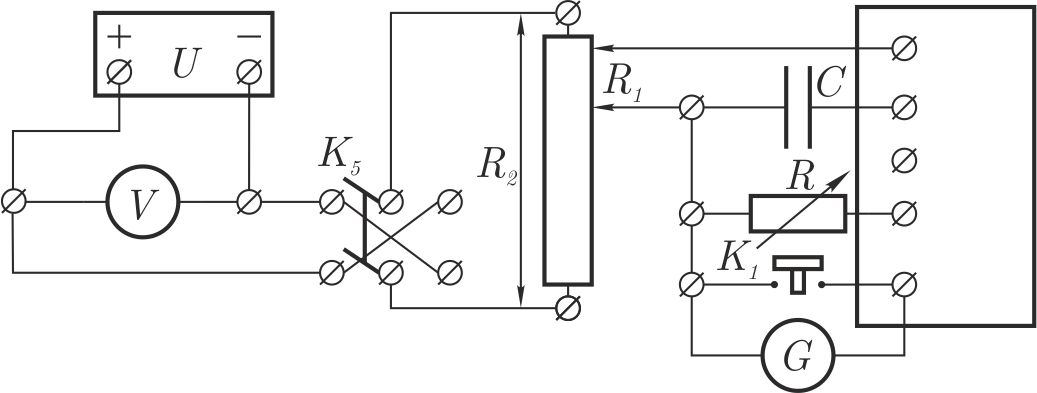
\includegraphics[width = 0.47\textwidth]{Sch2}
\captionsetup{justification = centering}
\caption{Схема установки для работы в баллистическом режиме} \label{Fig5}
\end{wrapfigure}

\textbf{Экспериментальная установка.} Схема для измерений в баллистическом режиме представлена на рис. \ref{Fig5}. В корбке с выводами находится сложная схема с кнопками для обеспечения правильных измерений. Емкость конденсатора $C = 2~\text{мкФ}$, $\frac{R_1}{R_2} = \frac{1}{40}$, и это отношение остается постоянным.

Заряд на конденсаторе выражается формулой 
\begin{equation}
q = CU_C = \frac{R_1}{R_2}UC
\end{equation}
При нажатии на кнопку этот заряд быстро проходит через гальванометр и сопротивление $R$, таким образом достигается баллистический режим. Если измерят угол отклонения так же, как и в части 2, то из (\ref{bal}) выражение для $C_q$ примет вид
\begin{equation}
C_Q = 2a\frac{R_1}{R_2}\frac{UC}{l_\text{max}},
\end{equation}
где $l_\text{max}$ - максимальное отклонение луча. Таким образом, в критическом режиме
\begin{equation}
{C_Q}_\text{кр} = 2a\frac{R_1}{R_2}\frac{UC}{{l_\text{max}}_\text{кр}}\label{cqcr}
\end{equation}

Из (\ref{rat}) в критическом режиме угол отклонения, а значит и $l_\text{max}$, в $e$ раз меньше, чем при отсутствии трения. Чтобы измерить $l_\text{max}$ в этом режиме (${l_\text{max}}_0$), измерим максимальное отклонение при отключенном от цепи гальванометре ${l_\text{max}}_1$ и декремент затухания $\Theta_1$. Тогда из определения декремента затухания следует, что
\begin{equation}
{l_\text{max}}_0 = {l_\text{max}}_1\cdot e^{\frac{\Theta_1}{4}}.\label{lmax0}
\end{equation}

После этого остается снять зависимость $l_\text{max}(R)$, и с помощью экстраполяции найти точку, в которой
\begin{equation}
l_\text{max} = \frac{{l_\text{max}}_0}{e}.
\end{equation}
Это удобно делать в координатах $l_\text{max}\left(\frac{1}{R+R_0}\right)$, т.к. несложно показать, что при $\gamma \ll \omega_0$, то есть при достаточно больших $R$, график в них линеен.

\textbf{Обработка данных.} Сначала проведем измерения при отключенном от цепи гальванометре. Для периода таких колебаний получим значение
\begin{equation}
T_0 \approx (6,43 \pm 0,02)~\text{с},
\end{equation}
этот результат получен из измерения времени 13 колебаний, время реакции принималось равным 0,2 с. Значение максимального отклонения 
\begin{equation}
{l_\text{max}}_1 \approx (21,3\pm0,2)~\text{см},
\end{equation}
значение следующего отклонения
\begin{equation} 
l_1 \approx (15,4\pm0,2)~\text{см}.
\end{equation}
Отсюда по определению
\begin{equation}
\Theta_1 = \ln\frac{l_1}{{l_\text{max}}_1} \approx 0,32\pm0,02.
\end{equation}
Таким образом, из (\ref{lmax0}) получим
\begin{equation}
{l_\text{max}}_0 \approx (23,1\pm0,2)~\text{см}.\label{lmax0val}
\end{equation}
Погрешность была вычислена по формуле
\begin{equation}
\Delta {l_\text{max}}_0 = {l_\text{max}}_0\frac{\Delta {l_\text{max}}_1}{{l_\text{max}}_1},
\end{equation}
т.к.
\begin{equation}
\Delta e^{\frac{\Theta_1}{4}} = \frac{\Delta\Theta_1}{4}e^{\frac{\Theta_1}{4}},
\end{equation}
а эта величина мала (относительная погрешность получится на порядок меньше $\frac{\Delta {l_\text{max}}_1}{{l_\text{max}}_1}$). Также теперь несложно найти ${l_\text{max}}_\text{кр}$:
\begin{equation}
{l_\text{max}}_\text{кр} = \frac{{l_\text{max}}_0}{e} \approx (8,5\pm0,1)~\text{см}. 
\end{equation}

Теперь снимем зависимость $l_{max}(R)$. Экспериментальные данные вместе с пересчитанными значениями занесены в таблицу \ref{tab3}.
\begin{table}[ht]\centering
\begin{tabular}{|*{10}{c|}}
\hline
$R,~\text{кОм}$&50&40&35&30&25&20&15&10&5\\
\hline
$l_\text{max},\text{см}$&17.1&16.4&15.9&15.3&15&14&12.3&10.4&7.1\\
\hline
$\frac{1}{R + R_0},~\text{Ом}^{-1}\cdot10^{-5}$&1.98&2.47&2.82&3.28&3.93&4.88&6.46&9.55&18.26\\
\hline
\end{tabular}
\caption{Данные для измерения $R_\text{кр}$ \label{tab3}}
\end{table}

\noindent Погрешность измерения $l_\text{max}$ принята 
\begin{equation}
\Delta l_\text{max} = 0,2~\text{см},
\end{equation}
погрешность измерения сопротивления считаем малой.
По этим данным построим график зависимости $l_\text{max}\left(\frac{1}{R+R_0}\right)$, он изображен на рис. \ref{Fig6}.

Хотя при больших $R$ зависимость действительно линейна, на всем измеренном диапазоне она хорошо аппроксимируется зависимостью вида $a\sqrt{x} + bx + c$ (такое фитирование и представлено на рис. \ref{Fig6}). Зная ${l_\text{max}}_\text{кр}$, находим точку, которая соответствует такому отклонению, это точка
\begin{equation}
G = \frac{1}{R + R_0} \approx (11,1\pm0,3)~\text{Ом}^{-1}\cdot10^{-5},
\end{equation}
погрешность была оценена по крайним значениям. Отсюда, т.к. эта точка критическая, находим $R_\text{кр}$:
\begin{equation}
R_\text{кр} = \frac{1}{G} - R_0 \approx 8,5 \pm 0,3~\text{кОм},
\end{equation}
погрешность была надена по формуле
\begin{equation}
\Delta R_\text{кр} = R_\text{кр}\frac{\Delta G}{G}.
\end{equation}
Осталось найти ${C_Q}_\text{кр}$ из выражения (\ref{cqcr}), получим
\begin{equation}
{C_Q}_\text{кр} = (1,98 \pm 0,04) \cdot 10^{-6}~\text{Кл},
\end{equation}
выражение для погрешности: 
\begin{equation}
\Delta {C_Q}_\text{кр} = {C_Q}_\text{кр}\sqrt{\left(\frac{\Delta U}{U}\right)^2 + \left(\frac{\Delta {l_\text{max}}_\text{кр}}{{l_\text{max}}_\text{кр}}\right)^2 + \left(\frac{\Delta a}{a}\right)^2}
\end{equation}

\begin{figure}[ht]\centering
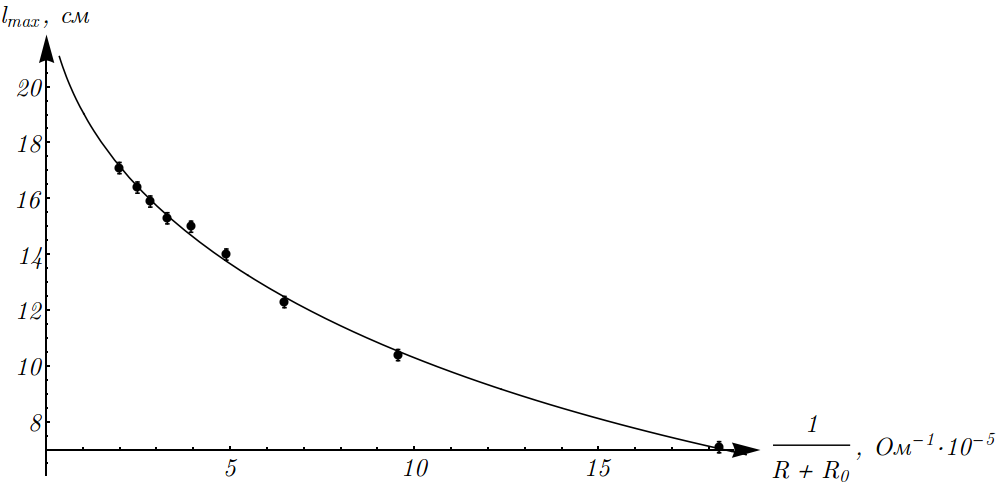
\includegraphics[width = 1\textwidth]{Plot3}
\captionsetup{justification = centering}
\caption{График зависимости $l_\text{max}\left(\frac{1}{R+R_0}\right)$\label{Fig6}} 
\end{figure}

Ранее в этой части был измерен $T_0$. Сравним его с величиной $R_0C$:
\begin{equation}
R_0C \approx 1~\text{мс} \ll T_0.
\end{equation}
\section{Заключение}
Мы измерили постоянные гальванометра, и, тремя разными способам, критическое сопротивление. Все они дали довольно близкие значения, но наибольшее отклонение от остальных у метода подбора (у двух оставшихся почти одинаковы результаты). Кроме того, мы сравнили характерное время разрядки с периодом колебаний, и получили, что его можно действительно считать малым.
\end{document} 
